\section*{Problem 1}
For the following signal:

\begin{figure}[H]
\caption*{}
\centering
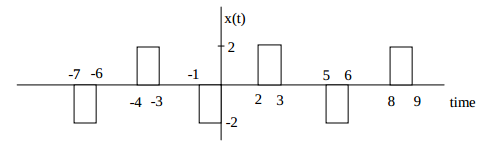
\includegraphics[width=0.8\textwidth]{figs/c1p1.png}
\label{fig:}
\end{figure} 

a) Find the Fourier series.

b) Plot the spectra versus frequency, $\omega = n \omega_0$.

\subsection*{Solution}
The period of the shown signal is $T=6$ and therefore $\omega_0 = \frac{2 \pi}{T} =  \frac{\pi}{3}$.

Taking the derivative of $x(t)$ we get:

\begin{figure}[H]
\caption{Derivative $\dot{x}$}
\centering
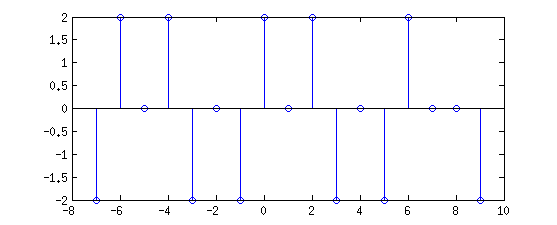
\includegraphics[width=0.8\textwidth]{figs/c1p1a.png}
\label{fig:}
\end{figure} 

The range t = [-3,3] contains one complete period of the signal. 
Usign (\ref{eq:c12}) we have:

\begin{equation*}
\begin{aligned}
\dot{x}(t) &= 2 (- \delta(t+1) + \delta(t) + \delta(t-2) - \delta(t-3) )\\
\end{aligned}
\end{equation*} 

The Fourier coefficients are obtained with:

\begin{equation*}
\begin{aligned}
j n \omega_0 X_n &= \frac{2}{6} \int_{-3}^3 (- \delta(t+1) + \delta(t) + \delta(t-2) - \delta(t-3) )e^{-j n \omega_0 t} \; dt\\
&= \frac{1}{3} (-e^{j n \omega_0} + 1 + e^{- 2 j n \omega_0} - e^{- 3 j n \omega_0}) \\
&= \frac{1}{3} [ 
	e^\frac{j n \omega_0}{2} ( e^\frac{- j n \omega_0}{2} - e^\frac{j n \omega_0}{2}) -
	e^\frac{-5 j n \omega_0}{2} ( e^\frac{- j n \omega_0}{2} - e^\frac{j n \omega_0}{2})] \\
&= \frac{1}{3} [ 
	( e^\frac{- j n \omega_0}{2} - e^\frac{j n \omega_0}{2}) 
	( e^{- j n \omega_0} (e^\frac{3 j n \omega_0}{2} - e^\frac{-3 j n \omega_0}{2}))] \\
&= \frac{4 j }{3} [ \sin \frac{n \omega_0}{2} \sin \frac{3 n \omega_0}{2} e^{- j n \omega_0 }] \\
X_n &= \frac{-4 j}{n \pi} [ \sin (n \frac{\pi}{6}) \sin (n \frac{\pi}{2}) e^{- j n \frac{\pi}{3}}] \\
\end{aligned}
\end{equation*} 

Next we use Matlab to plot the magnitude and phase of the spectra using the script given in \cite{wprobl_c1}

\zcodemat{sources/c1p1.m}{Calculate and plot magnitude and phase of Xn}

\begin{figure}[H]
\caption{Magnitude and Angle $X_n$}
\centering
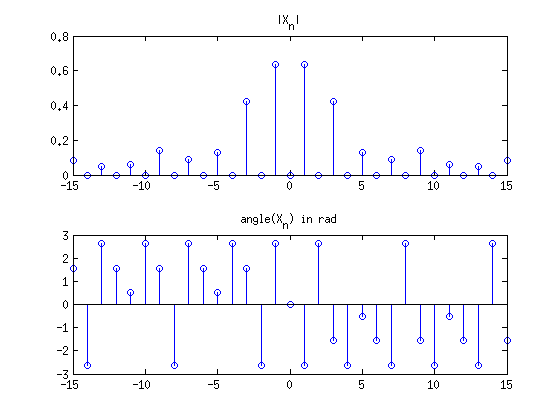
\includegraphics[width=0.8\textwidth]{figs/c1p1b.png}
\label{fig:c1p1b}
\end{figure} 

We then plot the approximation of the function using its Fourier coefficients 
\cite{wprobl_c1}.

\zcodemat{sources/fapprox.m}{Approximation of x(t) with Fourier coefficients}

We do this for N=5 and N=50:

\begin{figure}[H]
\caption{Approximation of x(t) by Xn}
\centering
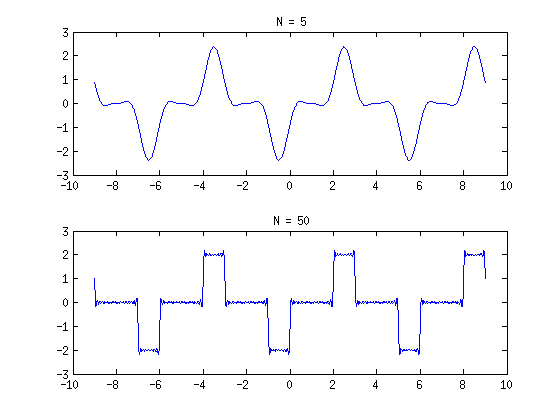
\includegraphics[width=0.8\textwidth]{figs/c1p1c.png}
\label{fig:c1p1c}
\end{figure} 

As we can see, the larger the N the more close to the original function we get. However, 
as a consequence of the Gibbs effect, we can't say that it'll be equal.
